\documentclass[aspectratio=169]{beamer}

\usetheme{Madrid}
\usecolortheme{default}

\usepackage[utf8]{inputenc}
\usepackage{booktabs}
\usepackage{graphicx}

\title{Loan Approval Prediction}
\subtitle{An End-to-End Machine Learning Pipeline}
\author{Ana Nicuesa}
\date{\today}

\setbeamertemplate{footline}[frame number]
\setbeamertemplate{navigation symbols}{}

\begin{document}

% ---------------------------------------------------------
\begin{frame}
    \titlepage
\end{frame}

% ---------------------------------------------------------
\begin{frame}{Agenda}
    \tableofcontents
\end{frame}

% ===========================================================
\section{Business Problem}

\begin{frame}{Business Problem}
    \begin{itemize}
        \item Manual loan underwriting is slow and inconsistent across reviewers.
        \item Goal: predict whether a loan application will be \textbf{approved} or \textbf{rejected}, using applicant and loan attributes.
        \item A reliable model can:
        \begin{itemize}
            \item Speed up decisions on straightforward applications
            \item Flag borderline cases for manual review
            \item Provide a consistent baseline to audit human decisions against
        \end{itemize}
        \item Approving a risky applicant and rejecting a creditworthy one have different costs $\rightarrow$ optimize for \textbf{ROC AUC}, not just accuracy.
    \end{itemize}
\end{frame}

% ===========================================================
\section{Dataset}

\begin{frame}{Dataset}
    \begin{columns}
        \begin{column}{0.55\textwidth}
            \textbf{563 loan applications}, 13 columns:
            \begin{itemize}
                \item Applicant: gender, marital status, dependents, education, self-employment
                \item Financial: applicant/coapplicant income, loan amount, loan term
                \item Credit history (meets guidelines: yes/no)
                \item Property area (urban / semiurban / rural)
                \item Target: \texttt{loan\_status} (approved / rejected)
            \end{itemize}
        \end{column}
        \begin{column}{0.45\textwidth}
            \textbf{Data quality issues found:}
            \begin{itemize}
                \item Missing values in \emph{every} column (3--6\%)
                \item Exact duplicate rows
                \item Repeated \texttt{loan\_id}s (resubmitted applications)
                \item Target missing in some rows
            \end{itemize}
        \end{column}
    \end{columns}
\end{frame}

% ===========================================================
\section{Exploratory Data Analysis}

\begin{frame}{Key Findings from EDA}
    \begin{itemize}
        \item Class balance: \textbf{71\% approved / 29\% rejected} $\rightarrow$ moderate imbalance
        \item \textbf{Credit history} is the strongest signal by far:
        \begin{itemize}
            \item Approval rate with good credit history: $\approx$80\%
            \item Approval rate without it: $\approx$11\%
        \end{itemize}
        \item Raw income and loan amount barely correlate with approval on their own
        \item Property area and marital status show smaller effects (semiurban and married applicants approved slightly more often)
        \item Income and loan amount are right-skewed with a few high-income outliers
    \end{itemize}
\end{frame}

\begin{frame}{Correlation with the Target}
    \centering
    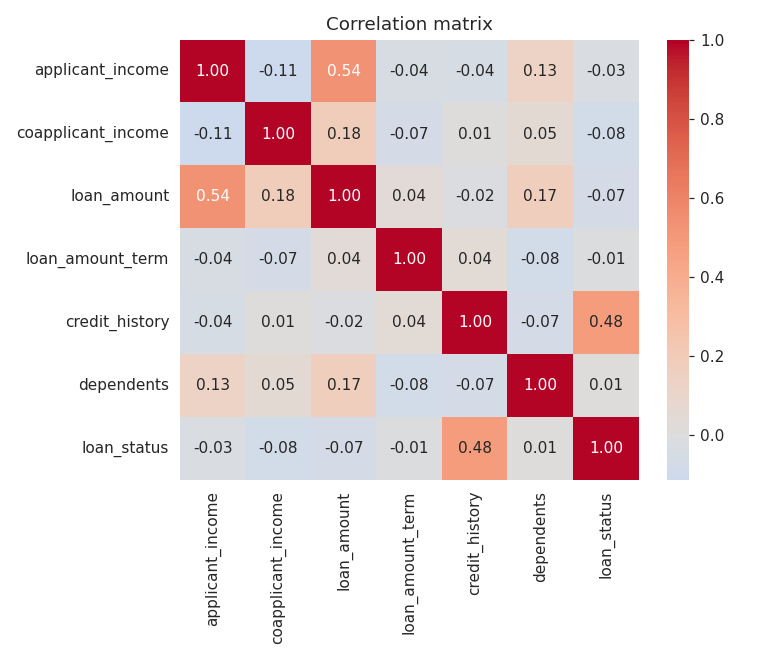
\includegraphics[width=0.55\textwidth]{../outputs/figures/correlation_heatmap.png}
\end{frame}

% ===========================================================
\section{Preprocessing \& Feature Engineering}

\begin{frame}{Preprocessing Pipeline}
    \begin{enumerate}
        \item \textbf{Cleaning:} drop exact duplicates, drop rows with missing target, drop identifier column, normalize \texttt{dependents} ("3+" $\rightarrow$ 3)
        \item \textbf{Feature engineering:}
        \begin{itemize}
            \item \texttt{total\_income} = applicant + coapplicant income
            \item \texttt{loan\_income\_ratio} = loan amount / total income
        \end{itemize}
        \item \textbf{Train/test split:} 80/20, stratified on target, fixed random seed
        \item \textbf{Imputation, scaling, encoding:} handled inside a \texttt{ColumnTransformer}, fit only on the training fold within cross-validation --- no leakage
        \begin{itemize}
            \item Numeric: median imputation + standard scaling
            \item Categorical: most-frequent imputation + one-hot encoding
        \end{itemize}
    \end{enumerate}
\end{frame}

% ===========================================================
\section{Modeling}

\begin{frame}{Modeling Approach}
    \begin{itemize}
        \item Three candidate models, each wrapped in the same \texttt{Pipeline} (preprocessing + classifier):
        \begin{itemize}
            \item Logistic Regression
            \item Random Forest
            \item XGBoost
        \end{itemize}
        \item 5-fold \textbf{stratified cross-validation}, scoring on ROC AUC
        \item \textbf{GridSearchCV} for Logistic Regression (small search space)
        \item \textbf{RandomizedSearchCV} for Random Forest and XGBoost (larger, continuous search spaces)
        \item Best pipeline persisted with \texttt{joblib} for reuse in evaluation and deployment
    \end{itemize}
\end{frame}

% ===========================================================
\section{Results}

\begin{frame}{Model Comparison}
    \begin{table}
        \centering
        \small
        \begin{tabular}{lccccc}
            \toprule
            Model & Accuracy & Precision & Recall & F1 & ROC AUC \\
            \midrule
            \textbf{Random Forest} & 0.804 & 0.827 & 0.918 & 0.870 & \textbf{0.818} \\
            XGBoost & 0.814 & 0.865 & 0.877 & 0.871 & 0.776 \\
            Logistic Regression & 0.833 & 0.826 & 0.973 & 0.893 & 0.746 \\
            \bottomrule
        \end{tabular}
        \caption{Test-set performance, best model in bold}
    \end{table}
    \vspace{0.3cm}
    Random Forest selected as the production model based on ROC AUC.
\end{frame}

\begin{frame}{ROC Curve Comparison}
    \centering
    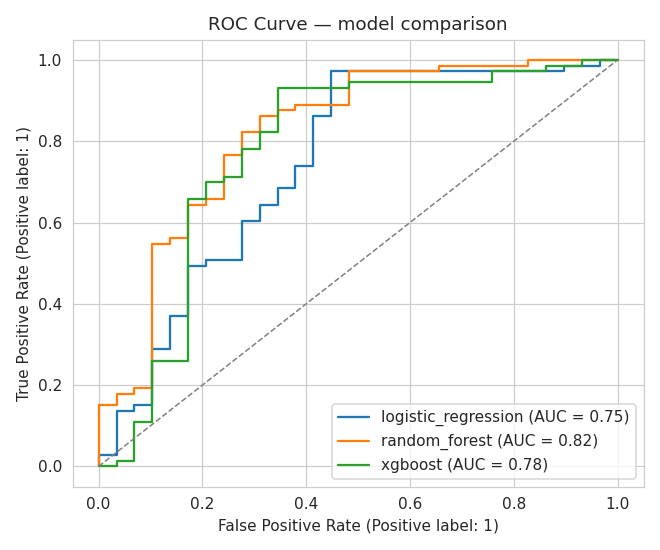
\includegraphics[width=0.55\textwidth]{../outputs/figures/roc_curve_comparison.png}
\end{frame}

\begin{frame}{Feature Importance --- Random Forest}
    \centering
    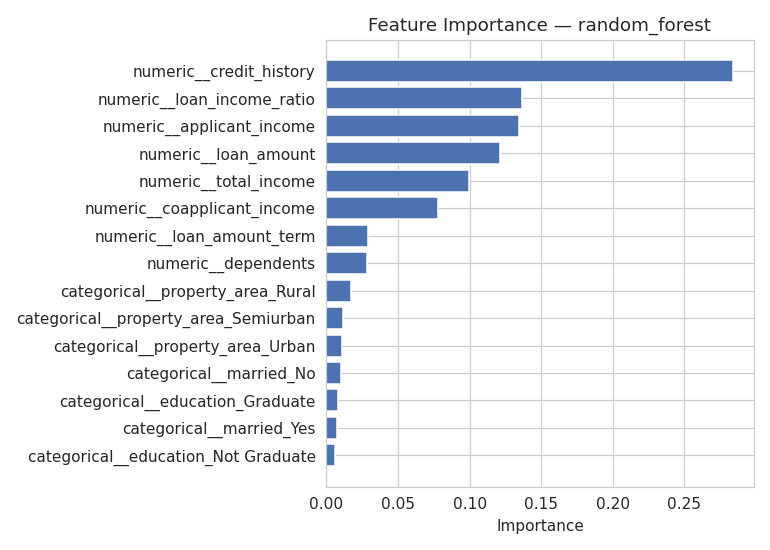
\includegraphics[width=0.65\textwidth]{../outputs/figures/feature_importance_random_forest.png}
    \vspace{0.2cm}

    \small Confirms the EDA: credit history dominates the prediction.
\end{frame}

% ===========================================================
\section{Explainability \& Fairness}

\begin{frame}{Model Explainability with SHAP}
    \begin{itemize}
        \item Feature importance shows \emph{what} matters; SHAP also shows \emph{which direction} and \emph{for whom}
        \item Global: mean absolute SHAP value bar chart + beeswarm plot (magnitude \emph{and} direction, per applicant)
        \item Local: waterfall plot per applicant, decomposing one prediction into feature contributions that sum exactly to the model's output
        \item SHAP mostly agrees with the Random Forest's built-in importance ranking, but adds direction, per-instance detail, and output-scale units --- impurity importance gives none of these
    \end{itemize}
\end{frame}

\begin{frame}{Global Feature Impact --- SHAP Beeswarm}
    \centering
    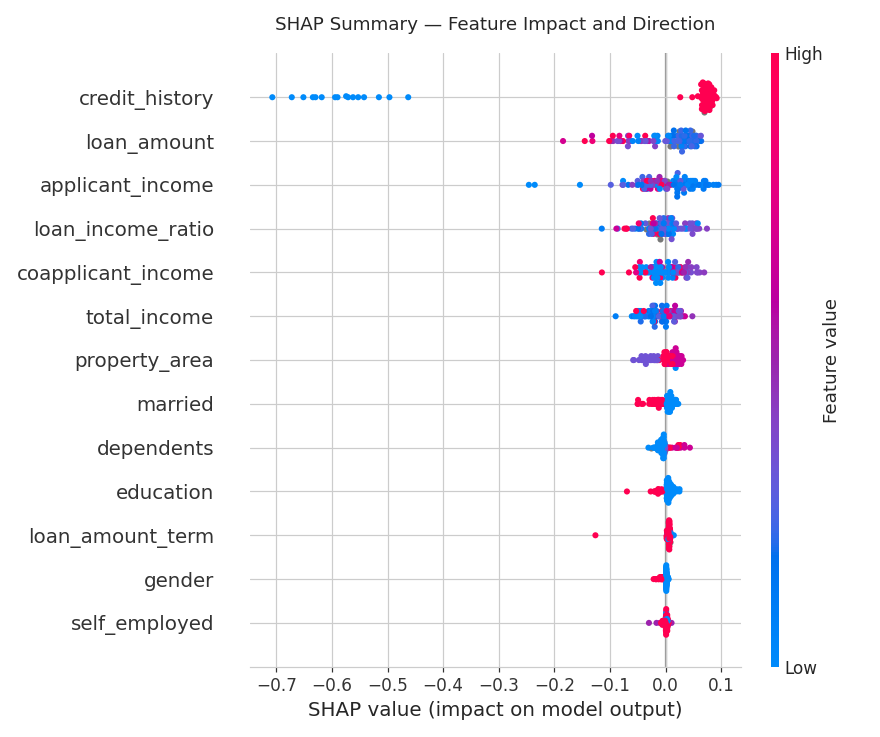
\includegraphics[width=0.5\textwidth]{../outputs/figures/shap_summary_beeswarm.png}

    \small Blue = low feature value, red = high. Credit history flips sign completely depending on its value.
\end{frame}

\begin{frame}{Local Explanations: Three Applicants}
    \begin{itemize}
        \item \textbf{Strong applicant} (credit history OK, solid income): approved, 95\% --- credit history and loan size drive it
        \item \textbf{Weak applicant} (no credit history, high loan request): rejected, 14\% --- credit history alone contributes $-0.46$
        \item \textbf{Borderline applicant} (modest income, good credit history): approved, 93\% --- credit history outweighs a middling loan-to-income ratio
    \end{itemize}
    \vspace{0.2cm}
    Same three profiles used in the Streamlit app's sanity checks and in \texttt{04\_Model\_Evaluation.ipynb} --- defined once in \texttt{src/utils.py}, no duplicated data.
\end{frame}

\begin{frame}{Important Caveat}
    \begin{itemize}
        \item SHAP explains what the \textbf{model} learned from historical data --- not a causal relationship in the real world
        \item A large SHAP value means the model relies on that feature; it does \emph{not} mean changing it would change a real applicant's outcome
        \item Correlated features (\texttt{applicant\_income}, \texttt{coapplicant\_income}, \texttt{total\_income}) can split credit for the same signal in ways that look inconsistent at a glance
        \item Training labels reflect \emph{past} approval decisions, which may themselves encode bias that SHAP will faithfully explain rather than correct
    \end{itemize}
\end{frame}

\begin{frame}{Fairness Check}
    \begin{itemize}
        \item \texttt{gender}, \texttt{married}, and \texttt{dependents} are present in the data and are sensitive attributes in real lending (ECOA in the US prohibits credit discrimination on sex and marital status)
        \item \texttt{gender} has the \textbf{lowest} mean absolute SHAP value of any feature in the model
        \item \texttt{married} and \texttt{dependents} show a small but non-zero effect --- well below \texttt{credit\_history} or the income features
        \item Risks that remain regardless: \textbf{proxy discrimination} (income correlates with marital status) and \textbf{historical bias} baked into the labels
        \item Conclusion: low SHAP magnitude is a useful signal, not a substitute for a legal/compliance fairness audit before real deployment
    \end{itemize}
\end{frame}

% ===========================================================
\section{Deployment}

\begin{frame}{Streamlit Application}
    \begin{itemize}
        \item Interactive web app for single-applicant predictions
        \item Inputs: gender, marital status, dependents, education, employment, income, loan amount/term, credit history, property area
        \item Output: \textbf{Approved / Rejected} with probability and confidence score
        \item Each prediction ships with a SHAP explanation: factors that increased vs.\ decreased approval probability, plus the full waterfall breakdown
        \item Same \texttt{predict.py} / \texttt{explain.py} logic used by the app and the notebooks --- no duplicated code
        \item Runs locally (\texttt{streamlit run app/app.py}) or from Google Colab
    \end{itemize}
\end{frame}

% ===========================================================
\section{Conclusions}

\begin{frame}{Conclusions \& Future Work}
    \textbf{Conclusions}
    \begin{itemize}
        \item Credit history is the single most predictive feature across every model
        \item Engineered affordability ratios add signal that raw income/loan figures don't provide
        \item Random Forest offers the best trade-off between recall and overall discrimination (ROC AUC)
    \end{itemize}
    \vspace{0.3cm}
    \textbf{Future improvements}
    \begin{itemize}
        \item Formal fairness audit (demographic parity, equal opportunity) beyond SHAP magnitude alone
        \item Larger hyperparameter search budget with more compute
        \item Larger, more recent dataset to validate generalization
        \item Data and SHAP-attribution drift monitoring if connected to a live pipeline
    \end{itemize}
\end{frame}

% ---------------------------------------------------------
\begin{frame}
    \centering
    \Huge Thank you
    \vspace{0.5cm}

    \normalsize Questions?
\end{frame}

\end{document}
